\chapter{\label{lesson11}Работа с Help}
{\bfseries Анонс:}\\\\
Проблемы инерционности. Работа с Help. Переменные. Движение прямо. Поворот на месте.\\\\
{\bfseries Цели:}
\begin{itemize}
	\item{}{\bfseries Обучающие:} Показать основные принципы работы с Help. Изучить, применить на практике и закрепить принципы работы с численными переменными в С.
	\item{}{\bfseries Коммуникативная:} Содействовать развитию у школьников самостоятельности мышления.\\
\end{itemize}	
{\bfseries Ход занятия:}\\\\
\begin{tabular}{lll}
	\hyperlink{lesson11x1}{1. Организационный момент} & Презентация & (15 мин)\\
	\hyperlink{lesson11x2}{2. Проблемы инерционности} & Презентация & (20 мин) \\
	\hyperlink{lesson11x3}{3. Практикум по проезду заданной длины} & Практикум & (30 мин) \\
	\hyperlink{lesson11x4}{4. Поворот на месте} & Практикум & 40 мин)\\
\end{tabular}\\\\

{\hypertarget{lesson11x1}{\blackBlueText{I. Организационный момент}}}\\\\ 

При изучении материала второго  раздела дети находятся за компьютером и после объяснения учителем каждого небольшого блока информации фронтально пробуют воспроизвести его действия самостоятельно и, при необходимости, опробовать код на стандартной трехколесной тележке, которая должна быть собрана в начале занятия.

Работа в третьем и четвертом разделе должна быть спланирована таким образом, что бы дать детям возможность самостоятельно, возможно в парах, попробовать решить задачу, получить подсказку и довести решение до конца.\\\\

{\hypertarget{lesson11x2}{\blackBlueText{II. Проблемы инерционности }}}\\\\

Второй способ решения проблемы инерционного прокручивания колес – это использовать специальную функцию nMotorEncoderTarget. Прежде чем обсудить, как работает именно эта функция, важно отметить общий механизм поиска неизвестных вам команд языка. Во всех программных средах вызов справки осуществляется нажатием клавиши F1. При этом вы попадаете в так называемый Help, документ, содержащий описание и примеры использования всех команд языка. Help  имеет оглавление, что позволяет удобно переходить к нужному разделу и искать необходимую информацию. Если вы примерно помните написание команды, но не помните ее синтаксис, то удобно воспользоваться поиском, набрав часть имени команды.

\begin{figure}[h!]
	\begin{center}
		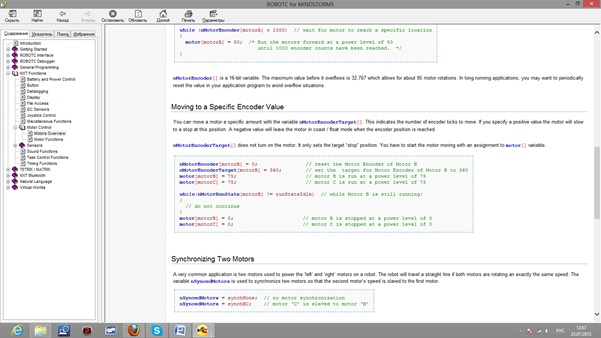
\includegraphics[width=0.95\linewidth]{chapters/chapter11/images/1}
		\caption{Вид Help в RobotC.}
		\label{ris:image11x1}
	\end{center}
\end{figure}

Итак, что же говорит нам Help про команду nMotorEncoderTarget? В качестве аргумента ему передается название соответствующего мотора, и ему можно присвоить значение, в градусах на которое должен повернуться этот мотор. При этом команда не выключит мотор самостоятельно, а лишь сменит свое значение на «стоп» в тот момент, когда нужно выключить моторы. Алгоритм расчета этого момента написан так, что бы выключить мотор чуть раньше и дать ему довернуться по инерции ровно до желаемого положения. Программа, поворачивающая колесо на 2 оборота будет выглядеть следующим образом:


{\programm
	{\slshape\bC{task main}}\rC{()}\\
	\rC{\{}\\
	\indent\bbC{nMotorEncoder}\rC{[\rrC{motorB}] = \rrC{0};}\\
	\indent\bbC{nMotorEncoderTarget}\rC{[\rrC{motorB}] = \rrC{720};}\\
	\indent\bbC{motor}\rC{[\rrC{motorB}] =  \rrC{75};}\\
	\indent{\slshape\bC{while}}\rC{(\bbC{nMotorRunState}[\rrC{motorB}] != \rrC{runStateIdle}) }\gC{// while motor B is still running}\\
	\indent\rC{\{}\\
	\indent\indent\gC{// do not continue}\\
	\indent\rC{\}}\\
	\indent\bbC{motor}\rC{[\rrC{motorB}] = \rrC{0};}\indent\gC{// motor B is stopped at a power level of 0}\\
	\rC{\}}\\
}\\\\	

В завершение разговора про инерцию, отметим, что при движении на средних скоростях в задачах, где нет нужды в очень точно позиционировании робота (объезды банок, помех), можно закрывать глаза на инерционный доезд робота.\\\\

{\hypertarget{lesson11x3}{\blackBlueText{III. Переменные. Практикум по проезду заданной длины}}}\\\\

Вспомним задачу, реализованную нами на прошлом занятии~--- проехать ровно 5 метров. Тогда пришлось опытным путем подбирать значение угла поворота колеса. Однако после этого мы обсудили, как можно вычислить проезжаемый путь, зная радиус колеса робота и угол поворота колеса. Решим обратную задачу.
Итак, пусть нам надо проехать путь \(s\), а радиус колеса робота \(r\). Тогда угол \(\varphi\), на который необходимо повернуть колесо:

\begin{equation}
s=2\pi r*\frac{\varphi}{360^{\circ}}\Rightarrow\varphi=\frac{360*s}{2\pi r}
\end{equation}

Можно самостоятельно вычислять по этой формуле каждый раз значение угла и подставлять в программу. Но гораздо удобнее считать это в самой программе, изменяя каждый раз лишь значение требуемого пути. Для этого можно написать следующую программу:
\clearpage
\begin{figure}[h!]
	\begin{center}
		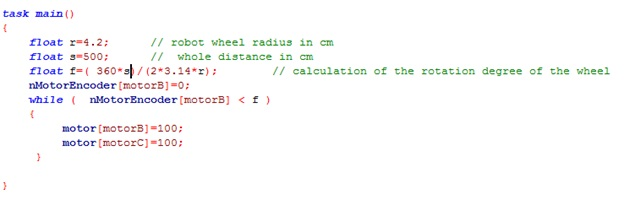
\includegraphics[width=1\linewidth]{chapters/chapter11/images/2}
		\caption{Вид Help в RobotC.}
		\label{ris:image11x2}
	\end{center}
\end{figure}

Логика программы нам понятна: мы вводим понятия радиуса колеса r, пути s и угла поворота f, и по выведенной формуле вычисляем требуемый угол поворота, который подставляется в цикл while. Но что значит float перед r,s,f?  Оказывается, что бы компилятор понимал введенные нами обозначения, или как принято говорить {\bfseries переменные} их надо {\bfseries объявить} в начале программы. При объявлении переменной прописывается ее тип, указывающий на то какого  рода значение будет храниться в переменной. Так, использованный нами тип float, указывает на то, что r,s,f могут принимать вещественные значения. Тип int мы будем использовать для целочисленных переменных.

{\slshape На начальном этапе изучения языка более подробная справка по типам данных только затруднит восприятие информации. При работе с детьми, изучавшими программирование до этого, можно подробнее остановиться на числовых типах данных в С и на преобразовании типов. В Приложении можно найти таблицу числовых типов данных языка С.}\\\\

{\hypertarget{lesson11x4}{\blackBlueText{IV. Поворот на месте}}}\\\\

Задача: Написать программу поворота робота на одном месте на 90 и 180 градусов (по вариантам) соответственно.

{\slshape Задача довольно сложная, поэтому для самостоятельного выполнения подходит только в сильных группах. В общем случае рекомендуется сначала обсудить следующее.}

При повороте тележки на месте, можно считать, что одно ее колесо неподвижно и на него не подается мощность, а второе колесо движется по дуге окружности радиуса \(l\), где \(l\)~--- расстояние между колесами тележки.\\\\

\greenText{Рис габарито тележки и дуг при повороте}\\\\

Тогда внешнее колесо должно пройти расстояние \(\Theta*l\), где \(\Theta\)~--- это угол, на который должна повернуться тележка. Подставляя это в формулу~\ref{formulRotateWheel} вместо \(s\), получаем:

\begin{equation}
\varphi=\frac{360*s}{2\pi r}=\frac{360*\Theta*l}{2\pi r}
\label{formulRotateWheel}
\end{equation}

где \(\varphi\)~--- угол на который должно повернуться внешнее колесо тележки. Итоговая программа имеет вид:

\begin{figure}[h!]
	\begin{center}
		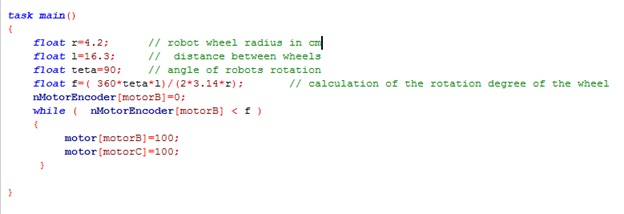
\includegraphics[width=1\linewidth]{chapters/chapter11/images/3}
		\caption{Вид Help в RobotC.}
		\label{ris:image11x3}
	\end{center}
\end{figure}

Обратим внимание, на то, что имена переменных могут состоять из многих символов. Поэтому при написании больших программ рекомендуется называть переменные так, чтобы было понятно, что в них содержится, без поиска комментария где-то вначале программы.